\documentclass{llncs}
\usepackage[T1]{fontenc}
\usepackage{lmodern}
\usepackage{hyperref}
\usepackage{cite} % Multiple citations in one \cite command
\usepackage{pgfplotstable}
\usepackage{array} % Required for pgfplotstable dec sep align
\pgfplotsset{compat=1.12}
\usepackage{booktabs}
\usepackage{todonotes}

\usepackage{enumitem}
\setlist{parsep=0pt, listparindent=0.5cm}

\begin{document}
\title{A Comparison of Parallel Graph Processing Benchmarks}
\author{Samuel D. Pollard \and Boyana Norris}
\institute{University of Oregon \\
	Eugene OR 97403, USA \\
	\email{spollard@cs.uoregon.edu} \\
	\email{norris@cs.uoregon.edu}
}
\maketitle
\begin{abstract}
The rapidly growing number of large network analysis problems has led to the emergence of many parallel and distributed graph processing systems---one survey in 2014 identified over 80. Since then, the landscape has evolved; some packages have become inactive while more are being developed. Determining the best approach for a given problem is infeasible for most developers. To enable easy, rigorous, and repeatable comparison of the capabilities of such systems, we present an approach and associated software for analyzing the performance and scalability of parallel, open-source graph libraries. We demonstrate our approach on five graph frameworks: GraphMat, the Graph500, the Graph Algorithm Platform, GraphBIG, and PowerGraph using synthetic and real-world datasets. We examine previously overlooked aspects of parallel graph processing performance such as phases of execution and energy usage for three algorithms: breadth first search, single source shortest paths, and PageRank and compare our results to Graphalytics.
\end{abstract}

\section{Introduction}

%% What's the problem (motivation)
Our research is motivated by the current state of parallel graph processing. The most comprehensive survey, released in 2014, identified and categorized over 80 different parallel graph processing systems, without considering domain specific languages \cite{Doekemeijer:2015:GPFSurvey}.

An overarching issue among these systems is the lack of comprehensive comparisons. One possible reason is the considerable effort involved in getting each system to run: satisfying dependencies and ensuring data are correctly formatted are generally nontrivial tasks. Additionally, some systems are developed with large, multi-node clusters in mind while others only work with shared memory, single node computers. An example of the former is GraphX \cite{Xin:2013:GraphX}, which incurs some overhead while gaining fault tolerance and an example of the latter is Ligra \cite{Shun:2013:Ligra}, a framework requiring a shared-memory architecture.
% ``The project was motivated by the fact that the largest publicly available real-world graphs all fit in shared memory''

From a graph algorithm user's point of view, there are optimizations for each system which may not be apparent. For example, the Parallel Boost Graph Library (PBGL)~\cite{Gregor:2005:PBGL} provides generic implementations of their algorithms and the programmer must provide the template specializations. The optimal data structures may differ across algorithms and graphs and must be determined by the programmer.

%% How do we address it?
To mitigate the inherent bias in hand-generated implementations, all the experiments performed use the author-provided implementations; we assume the developers of each system will provide the most performant implementation. While this limits the scope of the experiments it mitigates the bias inherent in our programming skills.

%To address the challenges of getting various systems installed, we automate the process as much as possible n
%To showcase our methods we analyze the performance of several graph processing benchmarks to facilitate the selection among such systems. Our analysis is done with minimal source code modification.

Our research contributions in this paper can be summarized as follows.
\begin{itemize}
	\item Automation of the installation, configuration, and dataset conversion to ensure the experiments execute in the same manner. Essentially, we provide a ``level playing field'' for graph algorithms.
	\item Comparison of algorithm runtime and scalability using several data sets.
	\item Comparison of our framework with the Graphalytics \cite{Capota:2015:Graphalytics} project.
	% BN: I think the bullet below is a bit too low-level for this summary, moving to later section.
	%\item Inspection of the source code of the surveyed parallel graph processing systems to ensure the same phases of execution are measured across differing execution and programming paradigms.
	\item An experimental framework distinguishing between the data structure generation and algorithm execution phases of each system.
	\item Analysis of energy consumption during the algorithm execution phase.
\end{itemize}

\section{Related Work}
A related project is Graphalytics \cite{Capota:2015:Graphalytics}, which also attempts to automate the setup and execution of graph packages for performance analysis. However, in order for Graphalytics to analyze a graph processing system---Graphalytics calls these platforms---a programmer must implement Java classes as wrappers to call the particular implementations, satisfy dependencies, and set the correct shell commands to execute. These all require some knowledge of the inner workings of each system in addition to familiarity with the Graphalytics API and involve a nontrivial amount of programming.

Moreover, the complexity of Graphalytics can obfuscate the true behavior of the program. By default, Graphalytics generates an HTML report listing the runtimes for each dataset and each algorithm in seconds. For example, one run of a single source shortest paths algorithm took 5.96 seconds. However, perusing the log files reveals a more complete picture: of these 5.96 seconds, 0.21 was spent computing the shortest paths while the remaining time consisted of building the necessary data structures. Furthermore, other performance-relevant details, such as the number of iterations run for PageRank, are not easily available using Graphalytics.
%We use GraphMat, the single source shortest paths algorithm, the dota-league dataset from the Game Trace Archive\cite{Guo:2012:GTA}, and the default settings as an example here.
% The full logs:
%Finished setting ids, time: 0.157009
%Starting sort
%Finished sort, time: 1.39571
%Finished setting edge pointers, time: 0.000133
%Starting build_dcsc
%Finished build_dcsc, time: 0.235948
%Finished setting ids, time: 0.154693
%Starting sort
%Finished sort, time: 1.75676
%Finished setting edge pointers, time: 0.000142
%Starting build_dcsc
%Finished build_dcsc, time: 0.238386
%Completed reading A from memory in 4.089144 seconds.
%Completed reading A from file in 5.114708 seconds
%Completed 19 iterations
%Timing results:
%- load graph: 5.11472 sec
%- initialize engine: 2.88486e-05 sec
%- run algorithm: 0.212451 sec
%- print output: 0.0799532 sec
%- deinitialize engine: 2.88486e-05 sec
%17:29:05.575 [INFO ] Benchmarking algorithm "Single source shortest paths" on graph "dota-league" took 5955 ms.

With a plugin to Graphalytics called Granula \cite{Ngai:2015:Granula}, one can explicitly specify a performance model to analyze specific execution behavior such as the amount of communication or runtime of particular kernels of execution. This requires in-depth knowledge of the source code and execution model. Furthermore, creating such a model requires a high level of expertise with the given system and with Granula\footnote{An example of Granula can be seen at \url{https://github.com/tudelft-atlarge/graphalytics-platforms-graphx/tree/master/granula-model-graphx}}.

As with Graphalytics, the initial development effort is high but Granula paired with Graphalytics allows automatic execution and compilation of performance results. Likewise, our approach provides automatic execution and performance analysis but without requiring a performance and execution model for each system.

Satish et al.~\cite{Satish:2014:NavigatingGraph} analyze the performance of several systems on datasets on the order of $30$ billion edges and \cite{Lu:2014:ExperimentalEval} uses six real-world datasets and focuses on the vertex-centric programming model.

Unlike these approaches, we focus on the \emph{depth} of analysis rather than the breadth via diversity of datasets or graph processing systems. We analyze  power and energy consumption in addition to details such as the number of iterations or the time to construct the data structures. Moreover, our approach requires little knowledge of the inner workings of each system; the data are collected using either hardware counter sampling of model-specific registers (for power) or through parsing log files (for execution time).

% The systems described in \cite{Doekemeijer:2015:GPFSurvey} operate with a wide range of parallelism paradigms and target architectures such as GPU \cite{Zhong:2014:Medusa, Kang:2009:Pegasus}, shared memory CPU \cite{Shun:2013:Ligra, kyrola:2012:Graphchi, Nguyen:2013:Galois}, a combination of CPU and GPU \cite{Gharaibeh:2012:Totem}, distributed filesystem based approaches \cite{Xin:2013:GraphX}, and distributed memory with MPI \cite{Gregor:2005:PBGL}.

% Beyond the systems described by Doekemeijer and Varbanescu, the problem has compounded with the addition of even more proprietary and open source projects such as \cite{Cheramangalath:2015:Falcon, Perez:2015:Ringo}, distributed memory approaches such as \cite{Hong:2015:PGX}. domain-specific languages \cite{Hong:2012:GreenMarl}, distributed database querying, \cite{Rodriguez:2015:Gremlin}, as well as novel communication schemes \cite{Edmonds:2013:ActiveMessages}. At the outset, this plethora of choices makes the question, ``which system is the best for my problem?'' daunting.

% In addition to libraries with associated APIs there has also been a propagation of ``reference implementations'' which implement the most common graph algorithms such as \cite{Beamer:2015:GAPBench, Nai:2015:Graphbig}. Thus, even selecting a standard and a benchmark over which to compare various implementations is nontrivial. To quote Andrew Tanenbaum, ``The nice thing about standards is that you have so many to choose from.''

\section{Experimental Setup}
We refer to a graph's \emph{scale} when describing the size of the graph. Specifically, a graph with scale $S$ has $2^S$ vertices. The datasets are described further in Sect.~\ref{sec:datasets}. We measure strong scaling and speedup by varying the number of threads from one to the total number of threads on our server, 72.

Each experiment uses 32 roots per graph. As with the Graph500, each root is selected to have a degree greater than 1. For PageRank, we simply run the algorithm 32 times. We plot many of the results as box plots with an implied 32 data points per box.

When possible, we measure the dataset construction time as the time to translate from the unstructured file data in RAM to the graph representation on which the algorithm can be performed. This is not possible for PowerGraph and GraphBIG because they read in the input file and build a graph simultaneously. The Graph500 builds the graph once and performs the BFS on each root in turn, speeding up experimentation but only giving a single data point for the dataset construction.

\subsection{Machine Specifications}
We performed experiments on our 36-core Intel Haswell server whose specifications are outlined below.
%Table~\ref{tab:specs} shows the specifications of the server on which we performed all experiments.
%\begin{table}[h!tb]
%	\centering
%	\caption{
The operating system is GNU/Linux version 4.4.0-22. The disparity between the CPU's advertised clock speed and the ``CPU Clock'' row is a result of the Turbo Boost technology which can increase the clock speed to a limit. We use the manufacturer's published maximum clock speeds which can be found at \url{http://ark.intel.com}.
\begin{center}
	% For arya I deleted Max RAM Freq	2133MHz
	\pgfplotstabletypeset[
	header=false,
	col sep=tab,
	string type,
	every head row/.style={output empty row, before row=\bottomrule},
	columns/0/.style={column type={|p{1in}|}},
	columns/1/.style={column type={p{3.2in}|}},
	every last row/.style={after row=\toprule},
	]{../report/specs.csv}
	%\label{tab:specs}
\end{center}

\subsection{Graph Processing Systems}

This study explores four shared memory parallel graph processing platforms. The first three are so-called ``reference implementations'' while the remaining two are included because of their performance and popularity. Our target is shared memory CPU processing. Other popular libraries such as the Parallel Boost Graph Library \cite{Gregor:2005:PBGL} are not considered here because the authors do not provide reference implementations. We consider the following systems.
\begin{itemize}
	\item The Graph500\footnote{We used the most recent version from \url{https://github.com/graph500/graph500}, most similar to release 2.1.4.} \cite{Murphy:2010:Graph500}, a set of large-scale graph benchmarks.
	\item The Graph Algorithm Platform (GAP) Benchmark Suite \cite{Beamer:2015:GAPBench}.
	\item GraphBIG \cite{Nai:2015:Graphbig} benchmark suite.
	\item GraphMat \cite{Sundaram:2015:GraphMat}, a high-performance graph library.
	\item PowerGraph \cite{Gonzalez:2012:Powergraph}, a framework for distributed graph-parallel computation on natural graphs.
\end{itemize}

Our approach is not specific or limited to these graph packages and can be extended to others with relatively modest effort (building each package and if necessary, instrumenting the different phases of the computation).

\subsection{Algorithms}\label{sec:algs}


We consider three algorithms: Breadth First Search (BFS), Single Source Shortest Paths (SSSP), and PageRank, although not all algorithms are implemented on all systems. We inspected the source code of the surveyed parallel graph processing systems to ensure the same phases of execution are measured across differing execution and programming paradigms. 

We select BFS because the canonical performance leaderboard for parallel graph processing is the Graph500 \cite{Murphy:2010:Graph500}. The advantage of the Graph500 is that it provides standardized measurement specifications and dataset generation. The primary drawback with the Graph500 is it measures a single algorithm.

Our work aims to add similar rigor to other graph algorithms by borrowing heavily from the Graph500 specification. The Graph500 Benchmark 1 (``Search'') is concerned with two kernels: the creation of a graph data structure from an unsorted edge list stored in RAM and the actual BFS\footnote{For a complete specification, see \url{http://graph500.org/specifications}}. We run the BFS using 32 random roots with the exception of PowerGraph which doesn't provide an reference implementation of BFS in its toolkits.

We select SSSP because of the straightforward extension from BFS; we need not modify the graph nor the root vertices from BFS.

PageRank is selected because of its popularity; most libraries provide reference implementations. One challenge with using PageRank is the stopping criterion; this is addressed in Sect.~\ref{sec:perf}. Verification of the PageRank results is beyond the scope of this paper, although this may explain some of the large performance discrepancies.

This approach is not specific to a particular algorithm; measuring the execution time, data structure construction time, and power consumption can be applied easily to other algorithms.

\subsection{Datasets}\label{sec:datasets}
We use the Graph500 synthetic graph generator which creates a Kronecker graph \cite{Leskovec:2010:Kronecker} with initial parameters of $A = 0.57, B = 0.19, C = 0.19,$ and $D = 1-(A+B+C) = 0.05$ and set the average degree of a vertex as 16. Hence, a Kronecker graph with scale $S$ has $2^S$ vertices and approximately $16 \times 2^S$ edges.

The Graphalytics results in Table~\ref{tab:graphalytics} were performed on the Dota-League dataset. This dataset contains 61,670 vertices and 50,870,313 edges. This dataset comes from the Game Trace Archive\cite{Guo:2012:GTA} and is modified for Graphalytics\footnote{This dataset is available at \url{https://atlarge.ewi.tudelft.nl/graphalytics/}.}. This dataset is useful because it is both weighted and more dense than the usual real-world dataset with an average out-degree of 824.

\section{Performance Analysis}\label{sec:perf}

We analyze the performance of the algorithms described in Sec.~\ref{sec:algs} in terms of execution time, scalability over multiple threads, and power and energy consumption.

\subsection{Runtime}

In Table~\ref{tab:graphalytics} we show the results from running Graphalytics on the Dota-League dataset. An explanation of each algorithm is given in \cite{Iosup:2016:Graphalyticstech}. Table~\ref{tab:graphalytics} shows only a broad overview of the two systems: GraphBIG and PowerGraph. In general, we see GraphBIG performs better. However, these preliminary results do not show the complete picture. For example, one may want to know the cost of performing additional computations on a graph once the data structures have been built. Additionally, one may desire runtime bounds to get a reasonable maximum timespan for a given problem.

%Table~\ref{tab:perf} lists performance in milliseconds of runtime according to the graphalytics output. Graphalytics also outputs MTEPS or millions of traversed edges pers econd. However, the graphalytics version does not make sense in all cases: for example, computing the local clustering coefficient involves traversing each edge multiple times (proportional to the sparsity of the graph), while BFS traverses each edge exactly once, and the number of edges traversed with PageRank depends on the connectivity of the graph and the number of iterations.

\begin{table}
% ,graphmat,openg,powergraph
%	Community Detection,0,212.5,1167
%	PageRank,0,293.5,983
%	Local Clustering Coefficient,0,316.5,1011
%	Weakly Connected Components,0,89,767.5
%	Single-Source Shortest Paths,11298.5,6378.5,34654.5
	\caption{Performance results are in milliseconds. Community detection is performed using label propagation. At the time of this writing, Graphalytics only supports SSSP for GraphMat.}
	\centering
	\pgfplotstabletypeset[
		col sep=comma,
		columns={[index]0,graphmat,openg,powergraph},
		every head row/.style={after row=\midrule},
		columns/0/.style={string type, column type={l|}, column name={}},
		columns/graphmat/.style={
			column name={GraphMat},
			string replace={0}{},
			dec sep align,
			empty cells with={N/A}
		},
		columns/openg/.style={
			column name={GraphBIG},
			dec sep align},
		columns/powergraph/.style={
			column name={PowerGraph},
			dec sep align}
	]{../report/runtime.csv}
	\label{tab:graphalytics}
\end{table}


\todo{rework this. It would be nice to compare Graphalytics and our approach on the real-world dataset.}
Table~\ref{tab:epg-perf}, by contrast, gives an overview of the performance results of running Graphalytics and our approach using the same dataset [TODO: Get the Dota-League Dataset working with easy-parallel-graph and replace Table~\ref{epg-perf}]. Table~\ref{tab:epg-perf} shows the average time across 32 roots, whereas Graphalytics by default shows results for a single root.

Figures~\ref{fig:bfs-time} and \ref{fig:sssp-time} show performance results for a Kronecker graph with scale $22$. The box plots give an idea of the runtime distributions. There is less variance in the runtimes of SSSP (between 0.1 and 1.7 seconds) compared to BFS (0.01 and 1.7 seconds) but GAP is the clear winner in both cases. The data structure construction times for GAP and GraphMat are consistent; in both cases the platforms create the same data structure for both algorithms. These results are consistent with \cite{Sundaram:2015:GraphMat} which lists GraphMat as more performant than PowerGraph in SSSP.

%\begin{table}
%	\centering
%	\begin{tabular}{l|c|c|c}
%		System & Load Graph & \begin{tabular}[x]{@{}c@{}}Construct Data \\ Structure\end{tabular} & Run BFS \\ \hline
%		Graph500 & 0.3474 & 0.3971 & 0.003380 \\
%		GAP      & 2.351  & 0.1935 & 0.001393 \\
%		GraphMat & 0.1511 & 1.101  & 0.1031 \\
%		GraphBIG & 37.22  & N/A    & 0.1528 \\
%	\end{tabular}
%	\caption{This table shows times for $2^{20}$ verties and the times are in seconds. The Graph500 generates the graph instead of loading it into a file. GraphBIG builds the graph and reads in the file simultaneously. These results were averaged across 32 roots.}
%	\label{tab:epg-perf}
%\end{table}

\begin{figure}
	\centering
	\begin{minipage}{0.48\linewidth}
		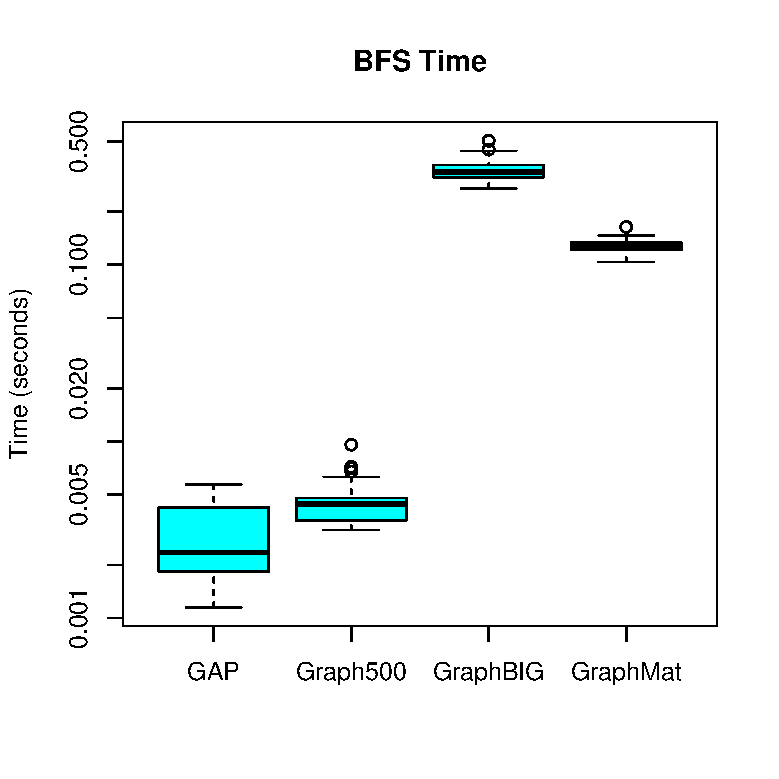
\includegraphics[width=\linewidth, trim=0 36pt 18pt 0, clip]{graphics/bfs_time.pdf}
	\end{minipage}
	\begin{minipage}{0.48\linewidth}
		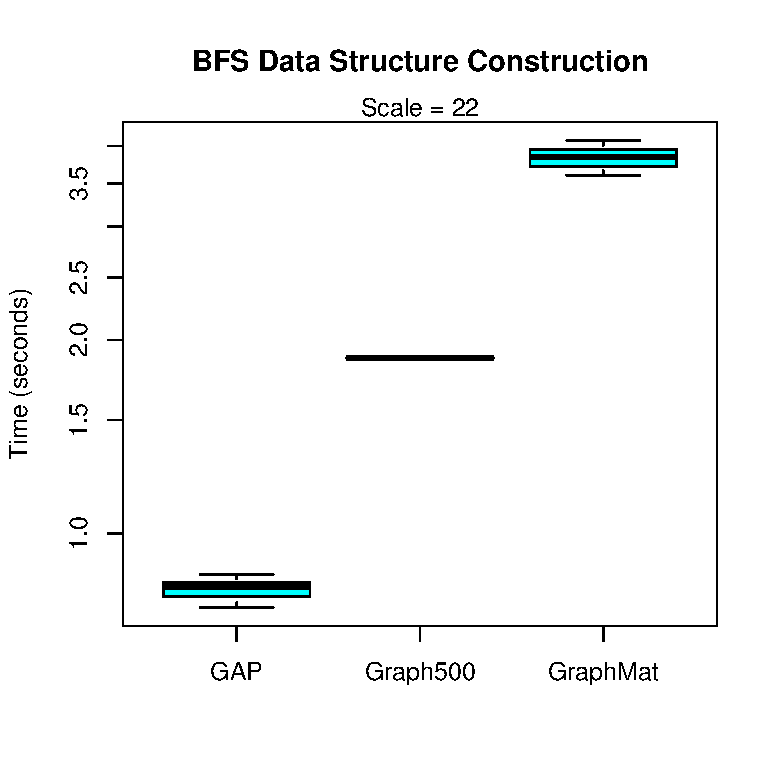
\includegraphics[width=\linewidth, trim=0 36pt 18pt 0, clip]{graphics/bfs_dsc.pdf}
	\end{minipage}
	\caption{The $y$-axes are logarithmic. The left box plot shows the time to compute BFS on 32 random roots while the right plot shows the times to construct the graph for each system. The Graph500 only constructs its graph once. GraphBIG reads in the file and generates the data structure simultaneously so is omitted.}
	\label{fig:bfs-time}
\end{figure}

\begin{figure}
	\centering
	\begin{minipage}{0.59\linewidth}
		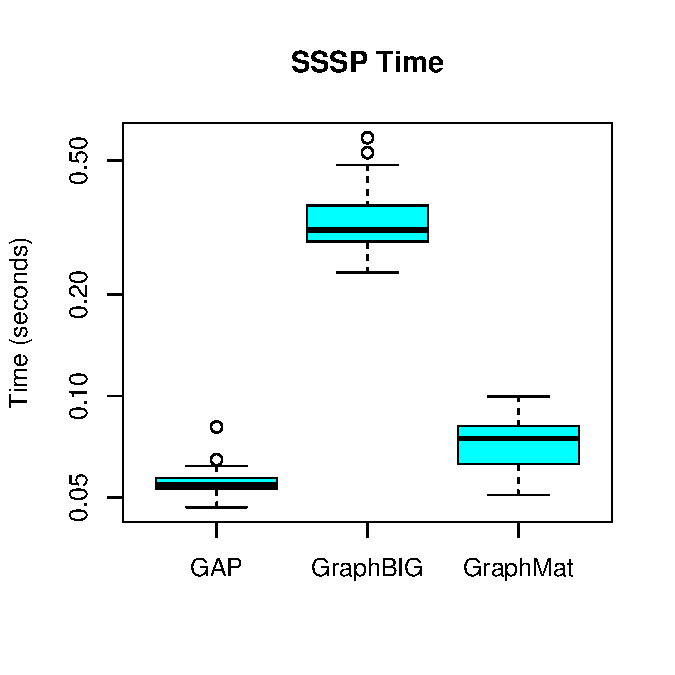
\includegraphics[width=\linewidth, trim=0 36pt 18pt 0, clip]{graphics/sssp_time.pdf}
	\end{minipage}
	\begin{minipage}{0.365\linewidth}
		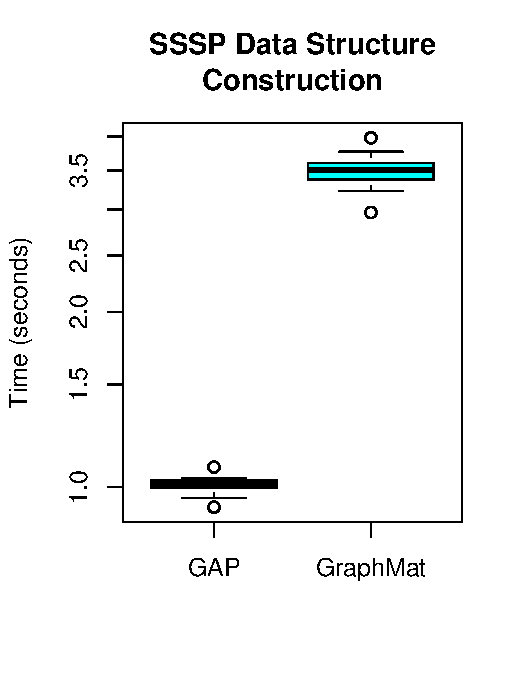
\includegraphics[width=\linewidth, trim=0 36pt 18pt 0, clip]{graphics/sssp_dsc.pdf}
	\end{minipage}
	\caption{The $y$-axes is logarithmic. The left box plot shows the time to compute the SSSP starting at the same 32 roots as Fig.~\ref{fig:bfs-time}. Both PowerGraph and GraphBIG construct their data structures at the same time as they read the file.}
	\label{fig:sssp-time}
\end{figure}

The behavior of PageRank is slightly different. As with SSSP and BFS, the GAP Benchmark Suite is the fastest but it also requires the fewest iterations.

We attempt to define similar stopping criteria for each system, but GraphMat executes until no vertices change rank; effectively its stopping criterion requires the $\infty$-norm be less than machine epsilon. This could account for the increased number of iterations. We adjusted the other systems to use $\sum_{k=1}^{n} |p_k^{(i)} - p_k^{(i-1)}| < \epsilon $ as the stopping criteria, where $i$ is the iteration and $n$ is the number of vertices. We use $\epsilon = 6 \times 10^{-8}$ because this value is approximately machine epsilon for a single precision floating-point number. The goal is to make the stopping criteria for all implementations as similar as possible.

Moreover, the logarithmic scale in Figures~\ref{fig:bfs-time} and~\ref{fig:pr} compresses the apparent variance in runtime. Each platform in Fig.~\ref{fig:pr} has a relative standard deviation between $1/4$ and $1/2$ that of the same system executing SSSP.


\begin{figure}
	\centering
	\begin{minipage}{0.48\linewidth}
		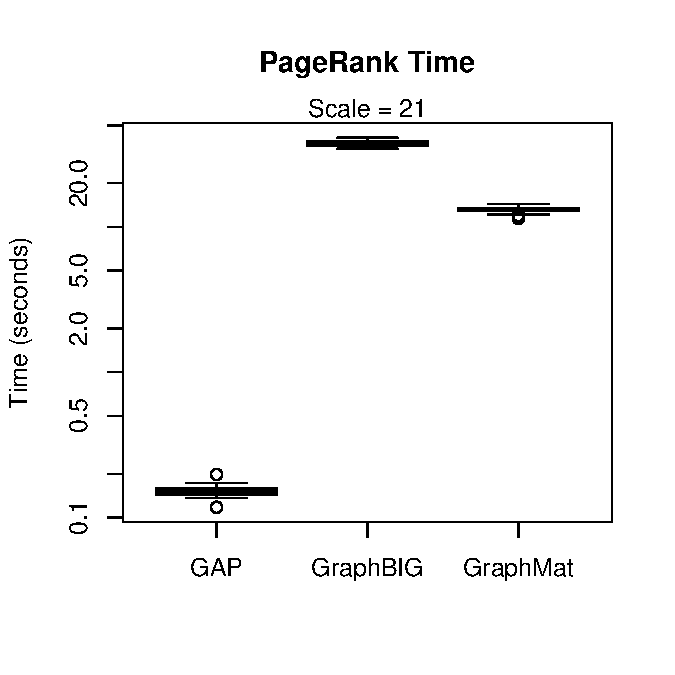
\includegraphics[width=\linewidth, trim=0pt 18pt 18pt 0pt, clip]{graphics/pr_time.pdf}
	\end{minipage}
	\begin{minipage}{0.48\linewidth}
		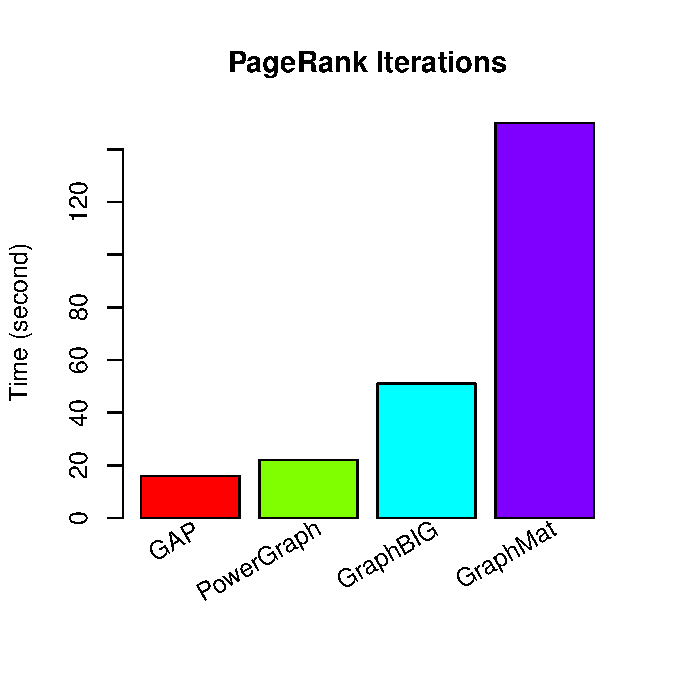
\includegraphics[width=\linewidth, trim=0 18pt 18pt 0pt, clip]{graphics/pr_iters.pdf}
	\end{minipage}
	\caption{The $y$-axis is logarithmic only for the left figure. GraphMat continues to run until none of the vertices' ranks change. For the others, we use the stopping condition that the sum of the changes in the weights is no more than $6 \times 10^{-8}$, or approximately machine epsilon for single precision floating point numbers.}
	\label{fig:pr}
\end{figure}

The difficulty in comparing iteration counts for PageRank underscores an important challenge for any comparison of graph processing systems. The assumptions under which the various platforms operate can have a dramatic effect on the program. For example, the GAP Benchmark Suite stores vertex weights as 32-bit integers. However, other systems store them as floating-point numbers. This may affect performance in addition to runtime behavior in cases where weights like $0.2$ are cast to $0$. Similarly, how a graph is represented in the system (e.g., weighed or directed) may have performance and algorithmic implications but is not always readily apparent.

Figure~\ref{fig:bfs-scaling} shows the scalability and speedup for BFS. We define the strong scaling as $T_1 / (n T_n)$ where $T_1$ is the serial time, $n$ is the number of threads, and $T_n$ is the time for $n$ threads. A linear scalability is when $T_n = T_1/n$ and is the horizontal line on the bottom plot in Fig.~\ref{fig:bfs-scaling}. These plots show in general poor scaling throughout, although GraphBIG has the best scaling. A potential explanation is that because GraphBIG is the slowest system, there is more room for improvement. Additionally, $2^{20}$ vertices is a ``small'' graph by today's standards and thus library designers focus on scalability for larger graphs. Another limitation may be the ability for OpenMP to efficiently handle such a large number of threads per machine.
\begin{figure}
	\centering
	\begin{minipage}{0.9\linewidth}
		% trim=left lower right upper
		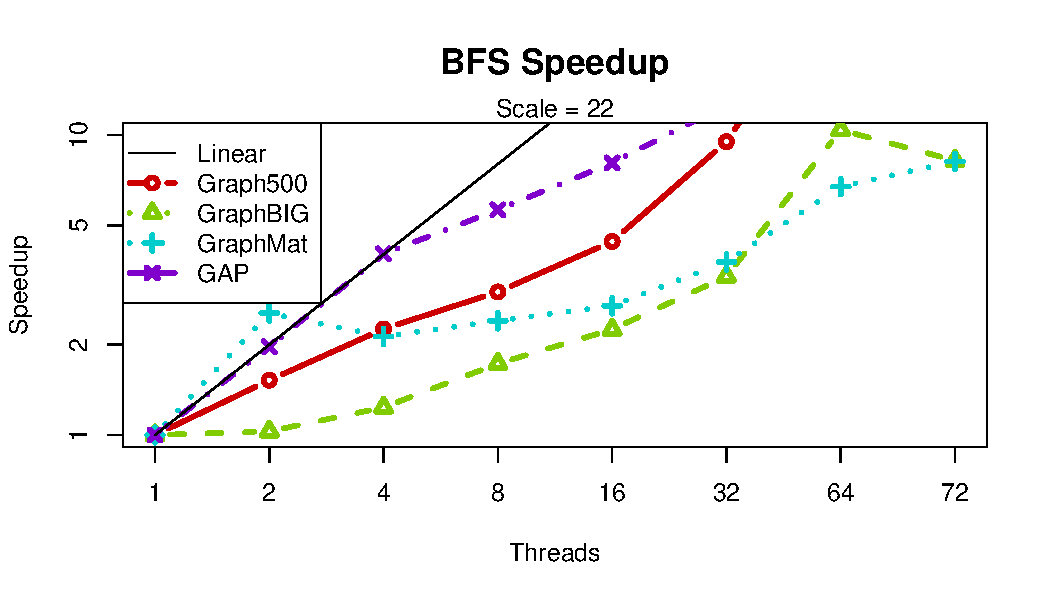
\includegraphics[width=\linewidth, trim=0 18pt 18pt 12pt, clip]{graphics/bfs_speedup.pdf}
	\end{minipage}
	\begin{minipage}{0.9\linewidth}
		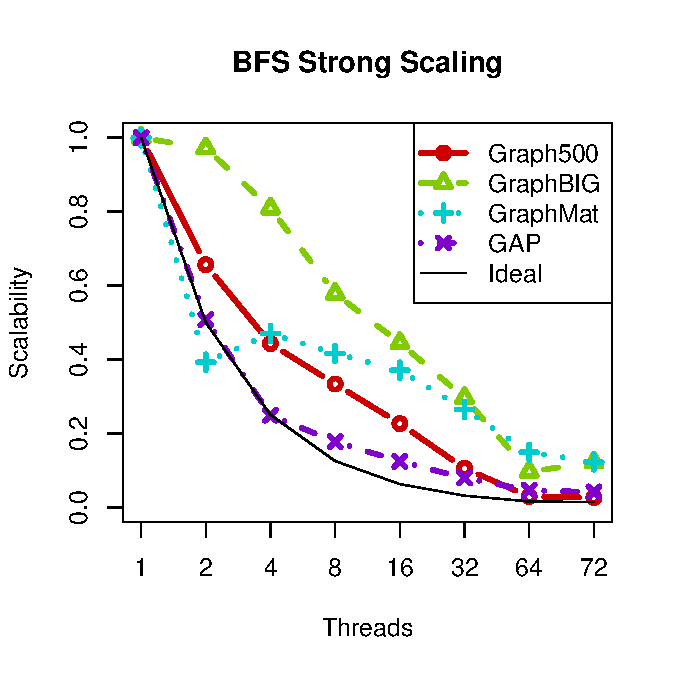
\includegraphics[width=\linewidth, trim=0 18pt 18pt 12pt, clip]{graphics/bfs_ss.pdf}
	\end{minipage}
	\caption{The top figure has both axes logarithmic with an exception at 72 threads for readability. Linear speedup is. GraphMat dips below 1 because it is slower for $2$ threads than for 1. $T_1$ is the serial time, $n$ is the number of threads, and $T_n$ time for $n$ threads.}
	\label{fig:bfs-scaling}
\end{figure}
\todo{Rerun GraphMat on scale 22 with 2 threads. Surprising that it slows down}

\subsection{Power and Energy Consumption}
We use the Performance Application Programming Interface (PAPI) \cite{Browne:2000:PAPI} to gain access to Intel's Running Average Power Limit (RAPL), which provides a set of hardware counters for measuring energy usage. We use PAPI to obtain average energy in nanojoules for a given time interval. We modify the source code for each project to time only the actual BFS computation and give a summary of the results in Table~\ref{tab:power}. In our case, the fastest code is also the most energy efficient, although with this level of granularity we could detect circumstances where one could make a tradeoff between energy and runtime.

\begin{table}
	\caption{The data are generated using a Kronecker graph with a scale of 22. Sleeping Energy refers to the power (in Watts) consumed during the \texttt{unistd} C \texttt{sleep} function, multiplied by the Time row. Essentially, this measures the amount of energy that would have been consumed if nothing was running. The increase over sleep is the ratio of the first and third columns. These are all averaged over 32 roots.}
	\centering
	\begin{tabular}{l|r|r|r|r}
			&	GAP  &    Graph500 & GraphBIG & GraphMat \\ \hline
		Time (s) &  0.01636 & 0.01884 & 1.600 & 1.424 \\
		Average Power per Root (W) & 72.38 & 97.17 & 78.01 & 70.12 \\
		Energy per Root (J) &	1.184 & 1.830 & 112.213 & 111.104 \\
		Sleeping Energy (J) & 0.4046  & 0.4660 & 39.591 &  35.234 \\
		Increase over Sleep & 2.926 & 3.928 & 2.834 & 3.153
	\end{tabular}
	\label{tab:power}
\end{table}

RAPL also allows the measurement of DRAM power, the results of which are shown in Fig.~\ref{fig:power}. The left plot describes the second row of Table~\ref{tab:power} in more detail. We notice a smaller spread of RAM power consumption, but still a noticeable difference. GraphMat exhibits the lowest average RAM power consumption (but not the shortest execution time). This information can be useful when choosing an algorithm to use in limited power scenarios, where a slower algorithms that will not exceed the power cap is preferred to a faster one that may exceed it.

\begin{figure}
	\centering
	\begin{minipage}{0.48\linewidth}
		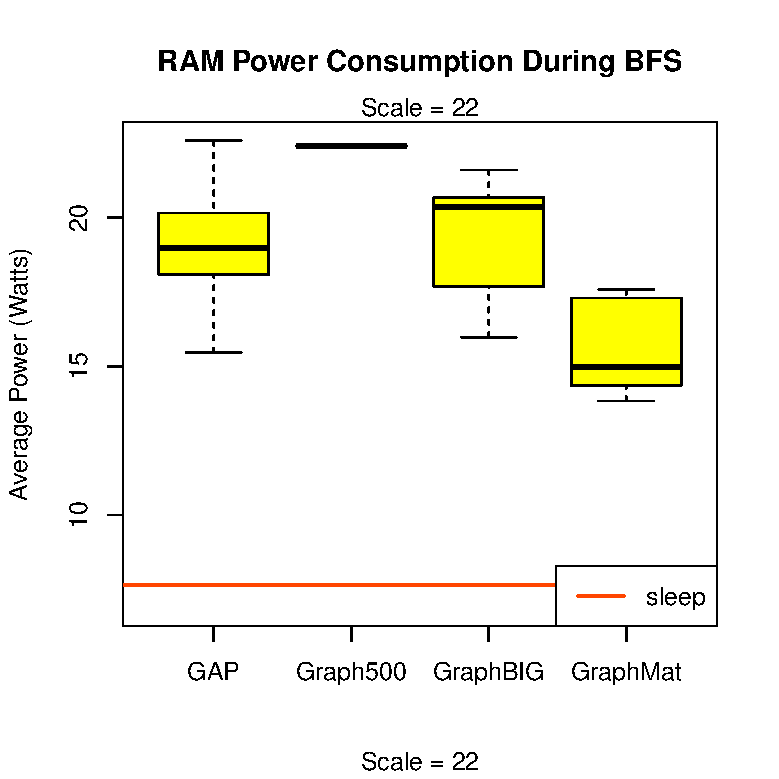
\includegraphics[width=\linewidth, trim=0 36pt 18pt 0, clip]{graphics/bfs_ram_power.pdf}
	\end{minipage}
	\begin{minipage}{0.48\linewidth}
		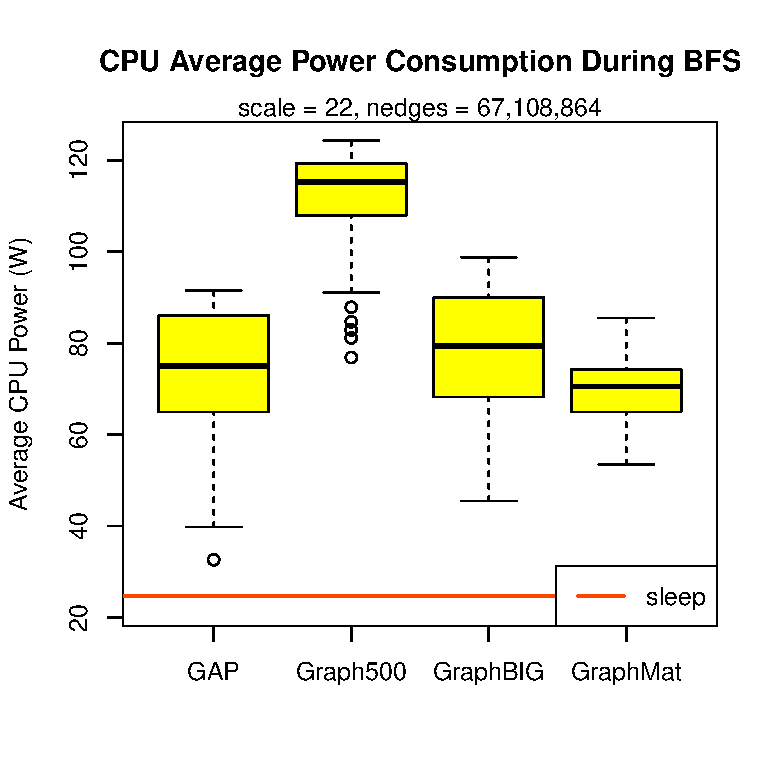
\includegraphics[width=\linewidth, trim=0 36pt 18pt 0, clip]{graphics/bfs_cpu_power.pdf}
	\end{minipage}
	\caption{Similar to Fig.~\ref{fig:bfs-time} we plot RAM and CPU Power Consumption for each of the 32 roots. Since the Graph500 runs multiple roots per execution, we only get a single datapoint. The baseline was computed by monitoring power consumption while a program containing only one call to the C \texttt{unistd} library function \texttt{sleep(10)} (ten seconds).}
	\label{fig:power}
\end{figure}

\section{Future Work and Conclusion}
We have presented a systematic approach to analyzing parallel graph processing performance, both measuring power consumption and the two fundamental phases of execution. While the comparison presented here can help one choose among alternatives for the selected packages and algorithms, the problem of selecting a graph processing framework for a given large-scale problem remains far from simple. Hence, we make our code available at \url{https://github.com/HPCL/easy-parallel-graph} and encourage further experimentation. Our results required minor changes to the original projects to add calls to PAPI sampling and those changes are also available on forked versions of the repositories. 

Overall, the GAP Benchmark Suite was the highest-performing system across the given datasets but the least scalable. However, this is only for relatively small graphs; all the graphs used here had at most $2^{22}$ vertices. It should be noted that GAP is also the most recent of projects. Thus, we recommend graph processing algorithm designers compare their implementations against the GAP Benchmark Suite as a good test of performance.

We found that GraphMat is not highly performant but does scale relatively well. One explanation is that GraphMat's underlying computation model (sparse matrix operations), paired the increased overhead of GraphMat's doubly-compressed sparse row (DSCR) graph representation, is better suited to larger-scale graphs.
% Furthermore, sparse matrix operations have been well studied so achieving good scalability is more realistic [cite]

Our work can continue in many directions. To ensure fairness, each platform must be configured to use the same graphs and the same roots. In the case of GraphBIG, this required the file to be loaded in for each experiment. By far the most time consuming of the experiments was GraphBIG's serial file input of uncompressed ASCII text format for graphs. This limited the sizes of the experiments we could run. Graphalytics also had circumstances with the more computationally expensive algorithms  where certain experiments fail \cite{Iosup:2016:Graphalyticstech}, so determining whether an algorithm will finish given a particular machine, input size, runtime limit, and resources is an important unanswered question we plan to pursue further.

\bibliographystyle{splncs03}
\bibliography{../drp}
\end{document}
